\subsubsection{ViewModels}
Herunder vil vi kort forklare de brugte viewmodels, i systemet.

\subsubsection{Klassebeskrivelser}
\textbf{CategoriesMenu}\\
CategoriesMenu er en menu med categorier. Denne klasse står for at kende alle kategorier. Ved et tryk på den categoryknappen vil CategoriesMenu oprette en menu med alle kategorier der eksisterer i systemet. Til hver menuitem vil den også tilknytte en liste af produkter. Derved kan der, ved tryk på menuitem, oprettes knapper med præcis de produkter der er ønsket. 

\begin{figure}[H]
	\centering
	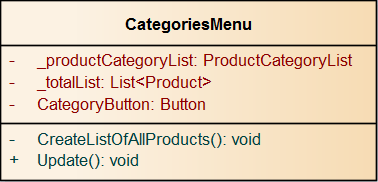
\includegraphics[width=0.3\textwidth]{Systemdesign/Frontend/pics/CategoriesMenu}
	\caption{CategoriesMenu.}
	\label{fig:PBC}
\end{figure}

\textbf{MenuCategory}
MenuCategory er en kategory i menuen. Den arver fra MenuItem som er et WPF element. Ved at oprette klassen på denne måde er det muligt at styre klassen direkte fra code behind. Derved kan der tilknyttes commands, og det muliggør dynamisk oprettelse af MenuItems.


\begin{figure}[H]
	\centering
	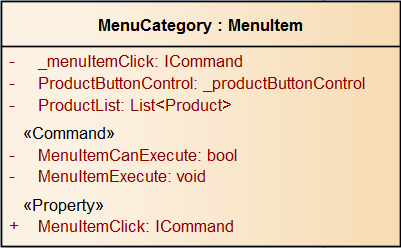
\includegraphics[width=0.3\textwidth]{Systemdesign/Frontend/pics/MenuCategory}
	\caption{MenuCategory.}
	\label{fig:PBC}
\end{figure}

\textbf{ProductButtonControl} \\
ProductButtonControl står for at styre hvilken knappeside der vises. Dette betyder at den indeholder en ProduktButtonList, der ved klik er i stand til at skifte knappeside.

\begin{figure}[H]
	\centering
	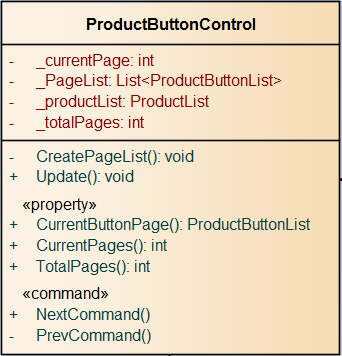
\includegraphics[width=0.3\textwidth]{Systemdesign/Frontend/pics/ProductButtonControl}
	\caption{ProductButtonControl.}
	\label{fig:PBC}
\end{figure}

\textbf{ProductButtonList} \\
ProductButtonList indeholder lister af knapper. Derved kan hver knappeliste symbolisere en side af knapper. Denne liste har ikke nogen anden funktionalitet, men eksisterer for at koden skal kunne facilitere dynamiske knappestørrelser i fremtiden. Denne klasse ville kunne tjekke på hvor stor siden er, og oprette knappesider med den ønskede antal knapper derefter.


\begin{figure}[H]
	\centering
	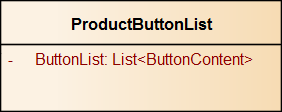
\includegraphics[width=0.3\textwidth]{Systemdesign/Frontend/pics/ProductButtonList}
	\caption{ProductButtonList.}
	\label{fig:PBL}
\end{figure}

\textbf{ProductButtonContent} \\
ProductButtonContent har indholdet af 1 knap på grænsefladen, samt produktinformationer og commands til at oprette produkter på shoppinglist ved tryk. Når man skifter side i grænsefladen produktbuttoncontent være forbundet til hver knap.

\begin{figure}[H]
	\centering
	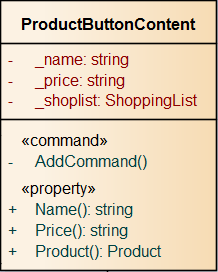
\includegraphics[width=0.2\textwidth]{Systemdesign/Frontend/pics/ProductButtonContent}
	\caption{ProductButtonContent.}
	\label{fig:PBCon}
\end{figure}